\documentclass[12pt]{article}
\usepackage{graphicx}
\usepackage{float}
\usepackage{xcolor}
\usepackage[margin=1in]{geometry}
\usepackage{amsmath}

\newcommand{\myvspace}{\vspace{4mm} \noindent}

\newcommand{\mytitle}[1]{\vspace{3mm} \noindent {\bf #1}~~}

\begin{document}
%\pagestyle{empty}

\begin{center}
\bf ASTR150 Exoplanet Lab
\end{center}

Planets orbiting stars in other solar systems -- called {\bf exoplanets} -- sometimes appear to pass in front of their stars once per orbit. If you could use a super-powerful telescope that could ``zoom in'' far enough, you would be able to see the planet eclipse the star. We don't have telescopes powerful enough to do this, so instead we carefully measure the brightness of the host stars and detect the small decrease in brightness that occurs when the planet blocks out a fraction of the star light once per orbit.  We call these eclipses {\bf transit} events, and this is how the majority of planets have been discovered to date, largely with NASA's {\it Kepler} spacecraft. 

The amount of light that a planet blocks out is related to how big the planet is. If the planet were the same size (had the same radius) as the star it would block out the star light completely when it passed in front, and if the planet were the size of a piece of dust it wouldn't block out much light at all. This means that we can measure the amount of light 

\begin{figure}[h!]
\centering
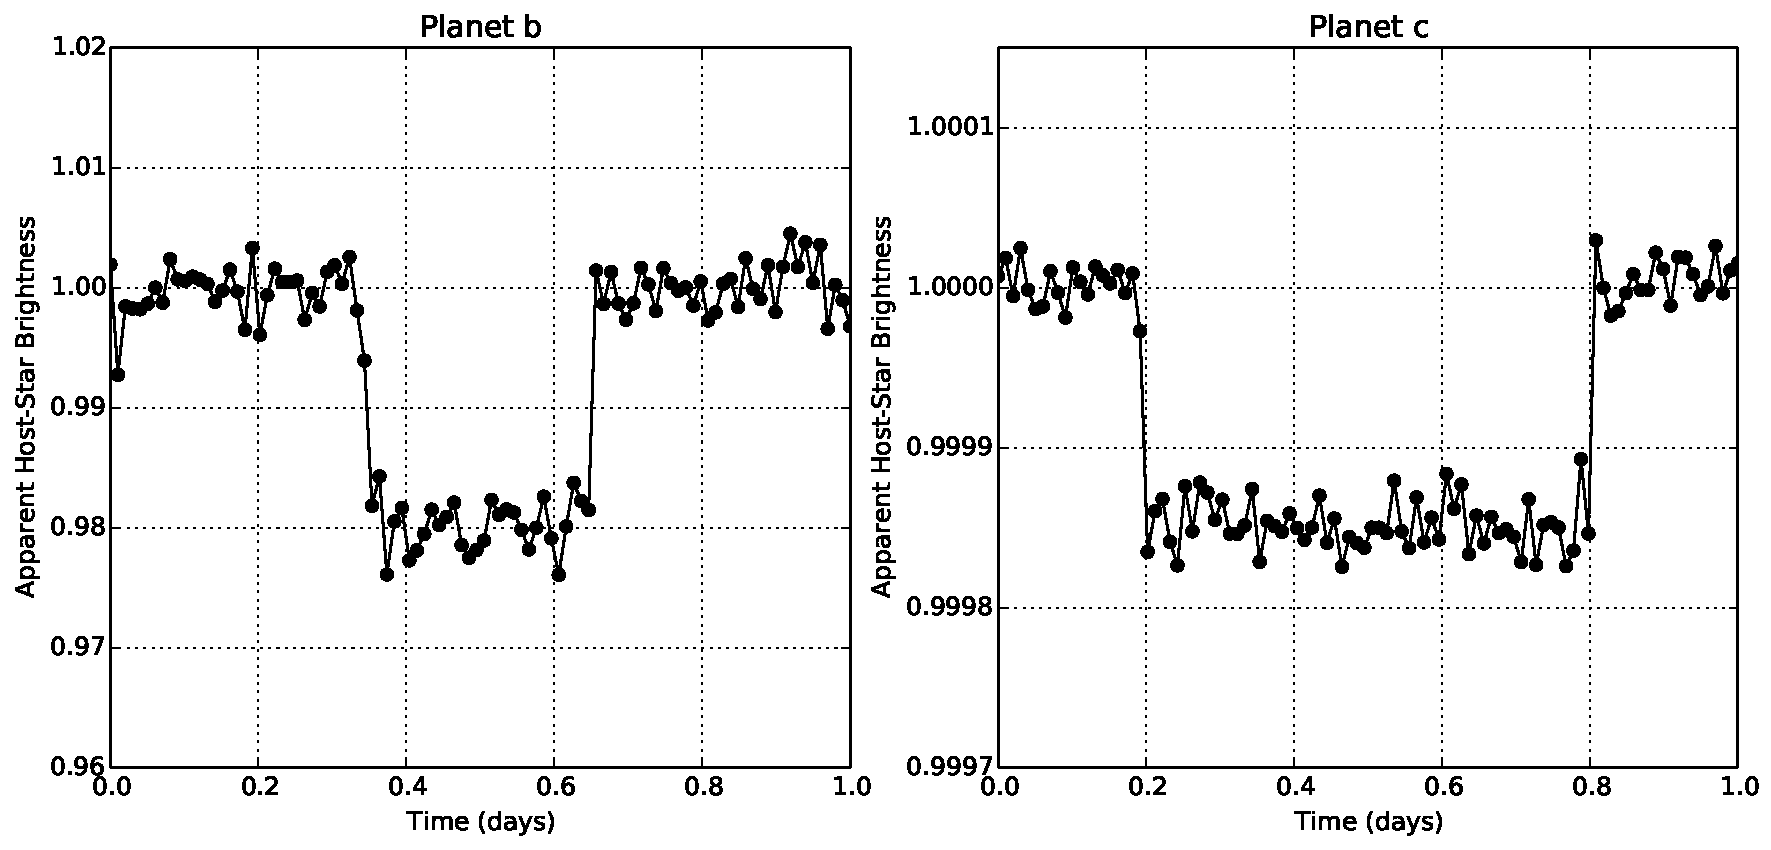
\includegraphics[scale=0.5]{plots/faketransit.pdf}
%\vspace{-5mm}
%\caption{Words words words}
\end{figure}

\end{document}